%&latex
%
\documentclass[../template.tex]{subfiles}
\usepackage{graphicx}

\begin{document}

\chapter{Stochastic Resonance}\lesson{9}{31/10/19}
The presence of noise in a system usually acts as a \textit{randomizing} perturbation, making its behaviour less regular, and more difficult to predict. In certain cases, however, the exact opposite can happen - meaning that \textit{noise can act as a stabilizer}. In particular, sometimes adding the \textit{right amount} of white noise \textit{boosts} a signal, leading  to a surprisingly higher \textit{signal-to-noise} (SNR) ratio. This is the phenomenon of \textbf{stochastic resonance} (SR).   

\section{Two-state model of SR}
To understand the main characteristics of \textit{stochastic resonance} we introduce an idealized two-state model, which will allow analytical computations to be made. 

\medskip

So, we consider a potential with two minima $s_1$ and $s_2$,\marginpar{Main concept} separated by a local maximum, as represented in fig. %insert figure
Consider a \textit{faint signal}, represented by a small perturbation of the potential, which rises and lowers the two minima in an alternate manner (fig. ). %insert figure 
Note that, in the absence of noise, a particle starting at rest in $s_1$ will not be able to reach $s_2$ due to the potential barrier - regardless of the modulation. On the other hand, if the particle is immersed in a thermal bath, random collisions can cause it to gain enough energy and make a transition to $s_2$. The probability of this happening will be higher when the potential barrier is lower, and so it will depend on the \textit{potential perturbation}, i.e. the signal. Then, measuring the frequency of transitions can lead to an estimate for the frequency of the underlying signal. 

However, if the noise is \textit{too} high, thermal fluctuations will cause transitions \textit{regardless} of the modulation, destroying the signal's effect. Ideally, we would want a noise amplitude $\sqrt{k}$ such that a transition $s_1 \to s_2$ is \textit{barely likely} when the potential barrier to surpass is at the \textit{minimum height}. 

\medskip

Let's make all this discussion quantitative.\marginpar{Quantitative discussion} Consider a particle of mass $m$ moving in a potential $V_0(x)$ with two minima $s_1$ and $s_2$, separated by a local maximum, as represented in fig. %insert figure
Besides the potential force $-V_0'(x)$, we introduce a viscous friction term $-\gamma \dot{x}$ and a \textit{random force} $\sqrt{k}\xi(t)$ representing the effect of thermal fluctuations. Let's see how this system behaves without any perturbation. \marginpar{\textbf{Unperturbed} system}

The equation of motion is given by:
\begin{align*}
    m \ddot{x} = - \gamma \dot{x} - V_0'(x) + \sqrt{k}\xi(t) \qquad 
\end{align*} 
where $\xi(t)$ is a \textit{white noise} function, i.e. such that $\langle \xi(t) \rangle = 0$ and $\langle \xi(t) \xi(t') \rangle = \delta(t-t')$.


Dividing by $\gamma$, in the overdamped limit $m/\gamma \ll 1$ we can ignore the acceleration term, leading to:
\begin{align} \label{eqn:langevin-sr}
    \dot{x} = -V_0'(x) + \sqrt{k}\xi(t) \Rightarrow \dd{x(t)} = -V_0'(x) \dd{t} +  \sqrt{k} \dd{B(t)}
\end{align}
The mean transition time\marginpar{Mean transition time} from $s_1$ ($x=-c$) to $s_2$ ($x=c$) is obtained by considering $x=-\infty$ as a \textit{reflecting boundary} and $x=c$ as an absorbing one, and then computing the time average of the survival probability for a particle starting at $-c$. This was already done in (\ref{eqn:sol1}, pag. \pageref{eqn:sol1}). To adapt that formula to the current case, we compare (\ref{eqn:langevin-sr}) with (\ref{eqn:langevin-escape}, pag. \pageref{eqn:langevin-escape}), which reads:
\begin{align*}
    \dd{x(t)} = \frac{F(x,t)}{\gamma} \dd{t} + \sqrt{2D(x,t)} \dd{B(t)}
\end{align*}
And so $\gamma = 1$, and $\sqrt{k} = \sqrt{2 D} \Rightarrow D = k/2$, meaning that $A(x) = -U'(x)/\gamma = -V_0'(x)$ (with $a=-\infty$ and $b=c$). This leads to:
\begin{align*}
    T_c(-c) &= \int_{-c}^c \dd{y} \int_{-\infty}^y \dd{z}\frac{2}{k} \exp\left(+\int_z^y \dd{v} \frac{2V'_0(x)}{k} \right) =\\
    &= \frac{2}{k} \int_{-c}^c \dd{y} \int_{-\infty}^y \dd{z} \exp\left(\frac{2}{k} V(y) - \frac{2}{k} V(z)  \right) =\\
    &= \frac{2}{k} \underbrace{\int_{-c}^c \dd{y} \exp\left(\frac{2}{k} V(y) \right)}_{I_1}   \underbrace{\int_{-\infty}^{y} \dd{z\exp\left(-\frac{2}{k} V(z) \right)}}_{I_2} 
\end{align*}
We can use the saddle-point method to compute both $I_1$ and $I_2$ (as we did in (\ref{eqn:Kramers-approx}, pag. \pageref{eqn:Karamers-approx}) - where now $D = 1/(\beta \gamma) \Rightarrow \beta = 2/k$ ). For $I_1$ the exponential argument is maximum at $y=0$ (the local maximum of $V$) and for $I_2$ at $z=c$ (the local \textit{minimum} of $V$, due to the $-$ sign). This leads to:
\begin{align*}
    T_c(-c) \approx \frac{2 \pi}{\sqrt{|V''(0)| V''(c)}} \exp\Big(\frac{2}{k} \underbrace{[V(0) - V(c)]}_{\Delta V} \Big)
\end{align*}
So, the \textit{transition rate}\marginpar{Unperturbed transition rate} in absence of perturbation (the signal) is:
\begin{align} \label{eqn:tran-rate-unperturbed}
    W_0 \equiv \frac{1}{T_c(-c)} \approx \frac{\sqrt{|V''(0)| V''(c)}}{2 \pi} \exp\left(-\frac{2}{k} \Delta V \right)  
\end{align} 
Note that:
\begin{itemize}
    \item The rate depends \textit{exponentially} on the ratio between the potential barrier height $\Delta V$ and the fluctuation amplitude $k$. As expected, a higher barrier means \textit{less}  transitions, while high noise means \textit{more} transitions.  
    \item The rate is proportional to the \textit{curvature} of the potential, both at the barrier ($V''(0)$) and at the destination ($V''(c)$). Intuitively, a higher $V''$ means that the potential is \q{spikier} at that point, and so has \q{lower width}, making the barrier more traversable. 
    \item The same exact result holds for the \textit{inverse transition rate} $1/T_{-c}(c)$, as the potential is symmetric. 
\end{itemize}
In this case, transition events are completely uncorrelated, and the system does not exhibit any regularity.

\medskip

We now add a \textit{small} \textit{periodic fluctuation} (the signal) to the potential:\marginpar{\textbf{Perturbed} system}
\begin{align*}
    V(x,t) = V_0(x) + V_1 \frac{x}{c} \sin(\omega_s t) \qquad V_1 \ll \Delta V
\end{align*} 
with period $t_s = 2\pi/\omega_s$. As the perturbation is linear, it does not change the second derivative of the potential. So we can use, at least in first approximation, the formula (\ref{eqn:tran-rate-unperturbed}):
\begin{align} \label{eqn:w12}
    W_{\substack{1 \to 2\\2 \to 1}} \approx  \frac{\sqrt{|V''(0)| V''(c)}}{2 \pi} \exp\left(-\frac{2}{k} (\Delta V \pm V_1 \sin(\omega_s t)) \right)
\end{align}
Note that now the transition rates are \textit{asymmetrical}, meaning that depending on time a change $s_1 \to s_2$ can be more likely than the opposite $s_2 \to s_1$.

We expect this system to exhibit some kind of regularity. To see this, we would have to \textit{follow} the movement of the particle, which is very difficult in the general case. So, in the following section, we \textit{reduce} the model to a simplified description.

\subsection{Reduced model}
Due to the presence of friction, the particle \textit{does not oscillate} around a minimum. So we expect it to remain close to $\pm c$ for most of the time, eventually transitioning to the other state. We assume these\marginpar{Discretization to two states} movements to happen \textit{almost instantaneously}, regarding all the \textit{in-between} positions as transients. So, we can \textit{forget} about all points except $\pm c$, thus \textit{discretizing} the system.

\begin{expl}
    This relies on the assumption that the timescale for the transitions is much longer than the timescale of relaxation on each well (i.e. the amount of time needed for the particle to \q{stop} at a potential minimum due to friction). This is indeed true in the \textit{overdamped} limit. 
\end{expl}

Denote with $W_1 \equiv W_{1 \to 2}$ and $W_2 \equiv W_{2 \to 1}$. Let $p_1 = \mathbb{P}(x=-c)$ be the probability of the particle being at $s_1$, and $p_2 = \mathbb{P}(x=c)$ that of being at $s_2$. Then the time evolution of the discretized system can be described by the following Master Equation:
\marginpar{\vspace{3em}Master Equation}
\begin{align*}
    \begin{cases}
        \dot{p}_1 = -W_1p_1 + W_2 p_2\\
        \dot{p}_2 = W_1 p_1 - W_2 p_2
    \end{cases}
\end{align*}
As we saw earlier, the transition probabilities $W_1$ and $W_2$ both depend on time.

By conservation of probability $p_2 = 1-p_1$, and so:
\begin{align} \label{eqn:p1diff}
    \dot{p}_1 = - W_1 p_1 + W_2(1-p_1) = -\underbrace{(W_2+W_1)}_{W} p_1 + W_2 = - W p_1 + W_2
\end{align}
The homogeneous case ($W_2=0$) is solved by separation of variables:
\begin{align*}
    \frac{\dd{p_1}}{p_1} = -W(t) \dd{t} \Rightarrow p_1(t) = \exp\left(-\int_{t^*}^t W(\tau) \dd{\tau}\right) 
\end{align*}
where $t^*$ is an arbitrary instant. The full solution of the inhomogeneous case, with initial condition $p_1(0) \equiv p_0$ is then:
\begin{align} \label{eqn:solp1}
    p_1(t) = \exp\left(-\int_{t_0}^t W(t') \dd{t'}\right) p_0 + \int_{t_0}^t \dd{t'} W_2(t') \exp\left(-\int_{t'}^t W(t'')\dd{t''}\right)
\end{align}

\begin{expl}
    Recall that the full solution of a differential equation $y' = A(t)y + b(t)$ with $y(t_0) = y_0$ is given by:
    \begin{align*}
        \varphi(t) = \Phi(t) \Phi(t_0)^{-1} y_0 + \Phi(t) \int_{t_0}^t \dd{\tau} \Phi(\tau)^{-1} b(\tau)
    \end{align*}
    where $\Phi(t)$ is any solution of the homogeneous equation.
\end{expl}
$W_1$ and $W_2$ are periodic functions with period $t_s$ (\ref{eqn:w12}):
\begin{align*}
    W_{1,2}(t+t_s) = W_{1,2}(t)
\end{align*}
Then, it is possible to show that (\ref{eqn:solp1}) reduces to an \textit{periodic solution} $p_1(t)^{\mathrm{as}}$ for $t \to \infty$ which is \textit{independent} on the initial condition $p_0$:
\begin{align}
    p_1(t)^{\mathrm{as}} = \frac{1}{1- \exp(-\langle W \rangle t_s) }  \int_0^{t_s} \dd{t'} W_2(t-t') \exp\left(-\int_{t-t'}^t \dd{t''} W(t'')\right) \label{eqn:periodic-asymptote}
\end{align}
In other words, after a certain amount of time, the system \q{forgets} everything about the initial state.

\begin{comment}
\begin{expl}
    \textbf{Derivation of (\ref{eqn:periodic-asymptote})}. We start by showing that the first term of (\ref{eqn:solp1}), where $p_0$ appears, vanishes for $t \to \infty$. We do this by summing and subtracting the mean $\langle W \rangle$ inside the exponential:
    \begin{align*}
        \exp\left(-\int_{t_0}^t W(t') \dd{t'}\right)p_0 = \exp\left(-\int_{t_0}^t [W(t') \textcolor{Red}{- \langle W \rangle + \langle W \rangle}] \dd{t'}\right)p_0 = \span\\
        &= \exp\left(-\langle W \rangle(t-t_0)\right) \exp\Big(-\int_{t_0}^t \underbrace{(W(t') - \langle W \rangle)}_{\delta W(t')}\dd{t'}\Big) p_0
    \end{align*}
    As $W=W_{1} + W_2$, with $W_{1,2}$ being probabilities in $[0,1]$, its mean is $>0$, and so this expression vanishes for $t \to \infty$.

    Then we need to remove the initial condition from the second term, where it appears as the dependence on $t_0$. To do this, we note that, thanks to periodicity, we can relate the integral over the $i$-th period to the integral over the first one. Explicitly, let's evaluate the second term of (\ref{eqn:solp1}) over a period $[t^*-2t_s, t^-t_s]$, and again add and subtract the mean $\langle W \rangle$ from the inner exponential:
    \begin{align}\label{eqn:I-1}
        I_{-1} &= \int_{t^* -2t_s}^{t^*-t_s} \dd{t'} W_2(t') \textcolor{Red}{e^{\langle W \rangle t'}} \exp\left(-\int_{t'}^t (W(t'') \textcolor{Red}{- \langle W \rangle})\dd{t''}\right)
    %\end{align*}
    \intertext{With a change of variable $t' \to t' - t_s$ we can \textit{shift} the domain of integration by one period:}
    %\begin{align*}
        &= \int_{t^*-t_s}^{t^*} \dd{t'} \underbrace{W_2(t'-t_s)}_{W_2(t')} e^{\langle W \rangle(t'-t_s)} \exp\Big(-\int_{t'-t_s}^t \underbrace{(W(t'') - \langle W \rangle)}_{\delta W(t'')} \dd{t''}\Big) \nonumber
    \end{align}
    Note that $W_2(t'-t_s) = W_2(t')$ thanks to periodicity, and also:
    \begin{align} \label{eqn:hshift}
        \int_{t'-t_s}^{t} \delta W(t'') \dd{t''} = \underbrace{\int_{t'-t_s}^{t'} \delta W(t'') \dd{t''}}_{0}  + \int_{t'}^t \delta W(t'') \dd{t''}
    \end{align} 
    where the first term is the integral of a periodic function $\delta W$ with $0$ mean over its period, and so it vanishes. Substituting back, we get:
    \begin{align*}
        I_{-1} = e^{-\langle W \rangle t_s} \underbrace{\int_{t^*-t_s}^{t^*} \dd{t'} W_2(t') e^{\langle W \rangle t'} \exp\left(-\int_{t'}^t \delta W(t'') \dd{t''}\right)}_{I_0}
    \end{align*}
    We denote with $I_n$ the integral with argument (\ref{eqn:I-1}) over the $n$-th period, i.e. $[t^*+(n-1)t_s, t^*+nt_s]$. So we found a relation between two \textit{consecutive} periods:
    \begin{align} \label{eqn:consecutive-shift}
        I_{-1} = e^{-\langle W \rangle t_s} I_0 \Rightarrow I_{n} = e^{-\langle W \rangle t_s} I_{n+1} \Rightarrow I_{n+1} = e^{\langle W \rangle t_s} I_n
    \end{align}
    where $t^*$ is an arbitrary \textit{reference time}. 

    By reiterating it, we can relate the $n$-th period to the first one:
    \begin{align*}
        I_{n+1} = e^{n\langle W \rangle t_s} I_1
    \end{align*} 
    Now, consider a $t \gg 1$. Then we can approximate the $[t_0,t]$ with that over \textit{all the $n$ periods} contained in it, i.e. $[t_0, t_0+n t_s]$, where $n = t/t_s$. Note that the relative error on $n$ \textit{vanishes} as $t \to \infty$. Then, denoting with $f(t')$ the argument of (\ref{eqn:I-1}):
    \begin{align*}
        \int_{t_0}^t f(t') \dd{t'} &= \int_{t_0}^{t_0+n t_s} f(t') \dd{t'} +\cancel{ \int_{t_0 + nt_s}^t f(t')\dd{t'}} =\\
        &\approx \int_{t_0}^{t_0 + t_s} f(t') \dd{t'} + \int_{t_0 + t_s}^{t_0+2t_s} f(t')\dd{t'} + \dots + \int_{t_0 + (n-1) t_s}^{t_0 + nt_s} f(t') \dd{t'} =\\
        &= I_1 + I_2 + \dots + I_n =\\
        &= I_1 + e^{\langle W \rangle t_s} I_1 + e^{2 \langle W \rangle t_s} I_1 + \dots + e^{(n-1) \langle W \rangle t_s} I_1 =\\
        &= I_1 \left(\sum_{j=0}^{n-1} (e^{\langle W \rangle t_s})^j\right) \underset{(a)}{=}  I_1\left(\frac{1 - e^{n \langle W \rangle t_s}}{1 - e^{\langle W \rangle t_s}} \right)
    \end{align*}
    where $n t_s \approx (t-t_0)$, $t^* = t_0$ and in (a) we used the formula for the partial sum of a geometric series.

    All that's left is to deal with $I_1$:
    \begin{align*}
        I_1 = \int_{t_0}^{t_0+ t_s} \dd{t'} W_2(t') e^{\langle W \rangle t'} \exp\left(-\int_{t'}^t \delta W(t'') \dd{t''}\right)
    \end{align*}
    We change variables $t_2 = t_0 - t' \Rightarrow t' = t_0-t_2$, shifting the integration path to $[-t_s,0]$:
    \begin{align*}
        I_1 &= -\int_0^{-t_s} \dd{t_2} W_2(t_0 - t_2) e^{\langle W \rangle(t_0 - t_2)} \underbrace{\exp\left(-\int_{t_0-t_2}^t \delta W (t'') \dd{t''}\right) }_{h(t_0-t_2, t)}=\\
        &= e^{\langle W \rangle t_0} \int_{-t_s}^0 \dd{t_2} W_2(t_0-t_2) e^{-\langle W \rangle t_2} h(t_0-t_2,t)
    \end{align*}
    Then we apply (\ref{eqn:consecutive-shift}) to shift the path to $[0,t_s]$:
    \begin{align*}
        I_1 = e^{\langle W \rangle t_0}  e^{\langle W \rangle t_s} \int_0^{t_s} \dd{t_2} W_2(t_0-t_2) e^{-\langle W \rangle t_2} h(t_0-t_2,t)
    \end{align*}
    Note that, due to periodicity:
    \begin{align*}
        W(t - t_2) = W(t \textcolor{Red}{-t_0 + t_0}-t_2) = W(nt_s + t_0 - t_2) = W(t_0-t_2)
    \end{align*}
    and the same argument holds for $h(t-t_2,t) = h(t_0-t_2,t)$ recalling (\ref{eqn:hshift}). So:
    \begin{align*}
        I_1 = e^{\langle W \rangle t_0}  e^{\langle W \rangle t_s} \int_0^{t_s} \dd{t_2} W_2(t_0-t_2) e^{-\langle W \rangle t_2} h(t_0-t_2,t)
    \end{align*}

\end{expl}
\end{comment}

The mean position is then:
\begin{align*}
    \langle x(t) \rangle^{\mathrm{as}} = -c p_1(t)^{\mathrm{as} } + c (1-p_1(t)^{\mathrm{as}}) = c(1-2p_1(t)^{\mathrm{as}})
\end{align*}

In this reduced description, we take $W_{1,2}$ to be \textit{constant} with an added small signal:
\begin{align*}
    \begin{cases}
        W_1(t) = \frac{W}{2} - \epsilon \sin (\omega_s t)\\
        W_2(t) = \frac{W}{2} + \epsilon \sin (\omega_s t) 
    \end{cases}
\end{align*} 

Denote $p_1(t) \equiv p$ for simplicity. Then, from (\ref{eqn:p1diff}) we have:
\begin{align*}
    \dot{p} = - Wp + \frac{W}{2} + \epsilon \sin(\omega_s t) = - W\underbrace{\left(p-\frac{1}{2} \right) }_{\Delta p}+ \epsilon \sin (\omega_s t)
\end{align*}
leading to:
\begin{align*}
    \dot{\Delta p} = - W \Delta p + \epsilon \sin(\omega_s t)
\end{align*}

If $\epsilon = 0$, the solution is:
\begin{align*}
    \Delta p(t) = \Delta p(0) e^{-W t}
\end{align*}

To \textit{quantify} how much $x(t)$ is \q{periodic}, we pass to frequency space with a Fourier transform. As we are interested in \textit{how much} each frequency contributes to the total signal, we consider the squared norm of the Fourier transform: \marginpar{Power spectrum}
\begin{align*}
    P(\omega) = \frac{1}{2 \pi \bar{t}} \left| \int_0^{\bar{t}} \dd{t} x(t) e^{-i \omega t} \right|^2
\end{align*}
where $\bar{t}$ is the time length of observation. $P(\omega)$ is the \textbf{power spectrum} of the process $x(t)$. In the limit $\bar{t} \to \infty$, we can use the Wiener-Khintchine theorem\index{Theorem!Wiener-Khintchine}\marginpar{\vspace{2em}Wiener-Khintchine theorem} to compute $P(\omega)$:
\begin{align*}
    P(\omega) = 4 \int_0^\infty \dd{\tau} C(t) \cos(\omega t)
\end{align*}
where $C(t)$ is the \textit{auto-correlation} function:
\begin{align*}
    C(\tau) = \frac{1}{t_s} \int_0^{t_s} \dd{t} \langle x(t+ \tau) x(t) \rangle^{\mathrm{as}}
\end{align*} 
As $x(t+\tau) x(t)$ effectively depends only on the \textit{time difference} between the arguments, $C(t) = \langle x(t)x(0) \rangle$. By direct computation, it can be found that:
\begin{align*}
    C(t) = c^2 e^{-W|t|}
\end{align*}
so that the power spectrum becomes: \marginpar{\vspace{1em}Unperturbed power spectrum}
\begin{align*}
    P^{(0)}(\omega) = 4c^2 \frac{W}{W^2 + \omega^2} 
\end{align*}
As can be seen in fig. \ref{fig:pw}, the power density remains constant up to the \textit{cut-off} frequency $W$, and then decreases. Note that there is no clear frequency that \q{dominates} over the others, meaning that the process is essentially irregular. 

\begin{figure} %to do 
    \centering
    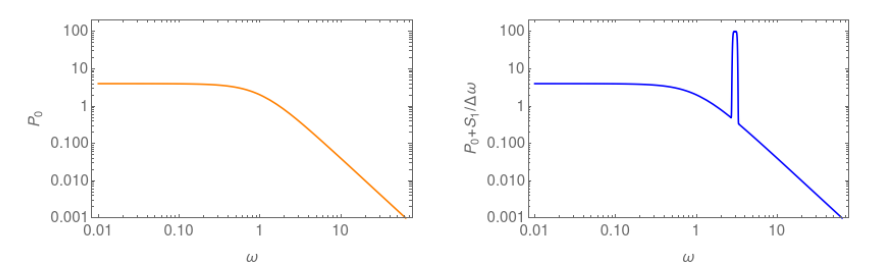
\includegraphics{image001.png}
    \caption{Power spectrum plot for $\epsilon = 0$ (left) and $\epsilon \neq 0$ (right)\label{fig:pw}}
\end{figure}






\end{document}
